% Options for packages loaded elsewhere
\PassOptionsToPackage{unicode}{hyperref}
\PassOptionsToPackage{hyphens}{url}
%
\documentclass[
]{article}
\usepackage{lmodern}
\usepackage{amssymb,amsmath}
\usepackage{ifxetex,ifluatex}
\ifnum 0\ifxetex 1\fi\ifluatex 1\fi=0 % if pdftex
  \usepackage[T1]{fontenc}
  \usepackage[utf8]{inputenc}
  \usepackage{textcomp} % provide euro and other symbols
\else % if luatex or xetex
  \usepackage{unicode-math}
  \defaultfontfeatures{Scale=MatchLowercase}
  \defaultfontfeatures[\rmfamily]{Ligatures=TeX,Scale=1}
\fi
% Use upquote if available, for straight quotes in verbatim environments
\IfFileExists{upquote.sty}{\usepackage{upquote}}{}
\IfFileExists{microtype.sty}{% use microtype if available
  \usepackage[]{microtype}
  \UseMicrotypeSet[protrusion]{basicmath} % disable protrusion for tt fonts
}{}
\makeatletter
\@ifundefined{KOMAClassName}{% if non-KOMA class
  \IfFileExists{parskip.sty}{%
    \usepackage{parskip}
  }{% else
    \setlength{\parindent}{0pt}
    \setlength{\parskip}{6pt plus 2pt minus 1pt}}
}{% if KOMA class
  \KOMAoptions{parskip=half}}
\makeatother
\usepackage{xcolor}
\IfFileExists{xurl.sty}{\usepackage{xurl}}{} % add URL line breaks if available
\IfFileExists{bookmark.sty}{\usepackage{bookmark}}{\usepackage{hyperref}}
\hypersetup{
  pdftitle={MBD - Estadística - Práctica 1a (ML)},
  pdfauthor={Arturo Menchaca y Víctor Juez},
  hidelinks,
  pdfcreator={LaTeX via pandoc}}
\urlstyle{same} % disable monospaced font for URLs
\usepackage[margin=1in]{geometry}
\usepackage{longtable,booktabs}
% Correct order of tables after \paragraph or \subparagraph
\usepackage{etoolbox}
\makeatletter
\patchcmd\longtable{\par}{\if@noskipsec\mbox{}\fi\par}{}{}
\makeatother
% Allow footnotes in longtable head/foot
\IfFileExists{footnotehyper.sty}{\usepackage{footnotehyper}}{\usepackage{footnote}}
\makesavenoteenv{longtable}
\usepackage{graphicx,grffile}
\makeatletter
\def\maxwidth{\ifdim\Gin@nat@width>\linewidth\linewidth\else\Gin@nat@width\fi}
\def\maxheight{\ifdim\Gin@nat@height>\textheight\textheight\else\Gin@nat@height\fi}
\makeatother
% Scale images if necessary, so that they will not overflow the page
% margins by default, and it is still possible to overwrite the defaults
% using explicit options in \includegraphics[width, height, ...]{}
\setkeys{Gin}{width=\maxwidth,height=\maxheight,keepaspectratio}
% Set default figure placement to htbp
\makeatletter
\def\fps@figure{htbp}
\makeatother
\setlength{\emergencystretch}{3em} % prevent overfull lines
\providecommand{\tightlist}{%
  \setlength{\itemsep}{0pt}\setlength{\parskip}{0pt}}
\setcounter{secnumdepth}{5}

\title{MBD - Estadística - Práctica 1a (ML)}
\author{Arturo Menchaca y Víctor Juez}
\date{Noviembre 22, 2020}

\begin{document}
\maketitle

\newpage
\tableofcontents
\newpage

\hypertarget{conjunto-de-datos}{%
\section{Conjunto de datos}\label{conjunto-de-datos}}

El conjunto de datos consta de las siguientes variables:

\begin{itemize}
\tightlist
\item
  id: identificador de la franja horaria (no guarda relación con el
  orden temporal)
\item
  year: año (2011 o 2012)
\item
  hour: hora del día (0 a 23)
\item
  season: 1 = invierno, 2 =primavera, 3 = verano, 4 = otoño
\item
  holiday: si el día era festivo
\item
  workingday: si el día era laborable (ni festivo ni fin de semana)
\item
  weather: cuatro categorías (1 a 4) que van de mejor a peor tiempo
\item
  temp: temperatura en grados celsius
\item
  atemp: sensación de temperatura en grados celsius
\item
  humidity: humedad relativa
\item
  windspeed: velocidad del viento (km/h)
\item
  count (sólo en el conjunto de entrenamiento): número total de
  alquileres en esa franja
\end{itemize}

A continuación mostramos la descriptiva de los datos:

\begin{verbatim}
##    year           hour       season   holiday  workingday weather 
##  2011:3879   Min.   : 0.00   1:1901   0:7466   0:2481     1:5122  
##  2012:3810   1st Qu.: 6.00   2:1920   1: 223   1:5208     2:1981  
##              Median :12.00   3:1943                       3: 586  
##              Mean   :11.57   4:1925                               
##              3rd Qu.:18.00                                        
##              Max.   :23.00                                        
##       temp           atemp          humidity        windspeed     
##  Min.   : 0.82   Min.   : 0.76   Min.   :  0.00   Min.   : 0.000  
##  1st Qu.:13.94   1st Qu.:16.66   1st Qu.: 46.00   1st Qu.: 7.002  
##  Median :20.50   Median :24.24   Median : 62.00   Median :12.998  
##  Mean   :20.27   Mean   :23.70   Mean   : 61.77   Mean   :12.802  
##  3rd Qu.:26.24   3rd Qu.:31.06   3rd Qu.: 77.00   3rd Qu.:16.998  
##  Max.   :41.00   Max.   :45.45   Max.   :100.00   Max.   :56.997  
##      count      
##  Min.   :  1.0  
##  1st Qu.: 41.0  
##  Median :145.0  
##  Mean   :191.4  
##  3rd Qu.:283.0  
##  Max.   :977.0
\end{verbatim}

\hypertarget{anuxe1lisis-de-las-variables}{%
\section{Análisis de las variables}\label{anuxe1lisis-de-las-variables}}

\hypertarget{categorizaciuxf3n-de-la-variable-hora}{%
\subsection{Categorización de la variable
hora}\label{categorizaciuxf3n-de-la-variable-hora}}

Descriptiva de la variable respuesta en función de la variable hora:

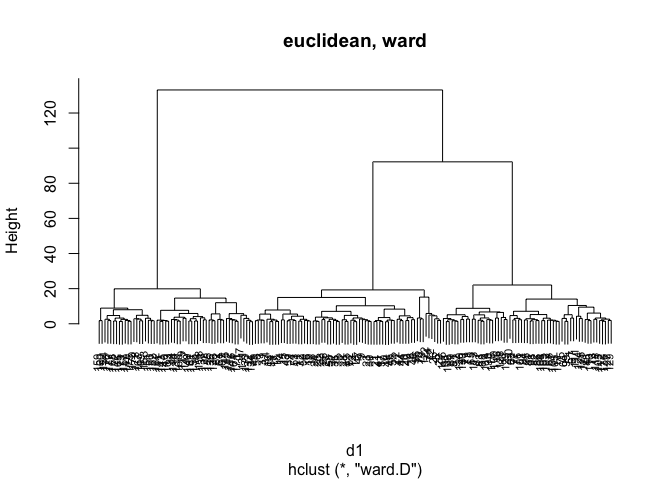
\includegraphics{informe_files/figure-latex/unnamed-chunk-4-1.pdf}

Decidimos agrupar la variable hora en los siguientes grupos:

\begin{itemize}
\tightlist
\item
  Morning: de 0:00h a 6:00h
\item
  Moving: de 7:00h a 8:00h y de 17:00 a 19:00
\item
  Worktime: de 9:00h a 16:00h
\item
  Night: de 20:00h a 23:00h
\end{itemize}

A continuación la descriptiva de la variable hora categorizada:

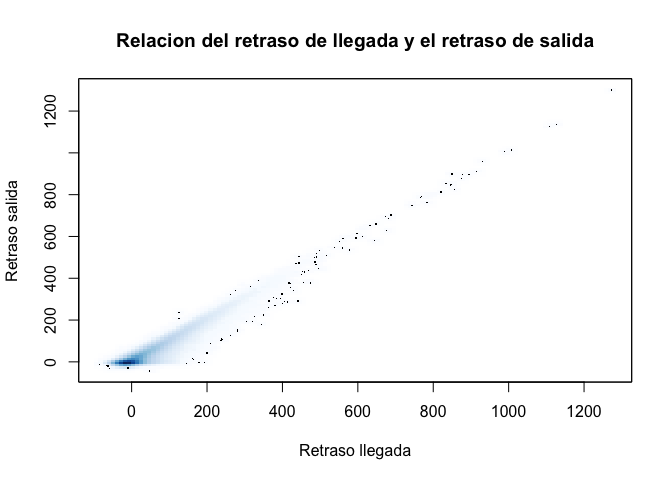
\includegraphics{informe_files/figure-latex/unnamed-chunk-5-1.pdf}

\hypertarget{descriptiva-de-las-variables-numuxe9ricas}{%
\subsection{Descriptiva de las variables
numéricas}\label{descriptiva-de-las-variables-numuxe9ricas}}

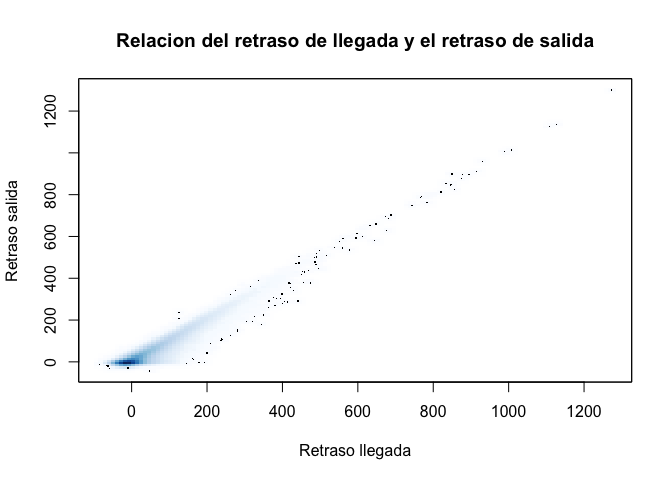
\includegraphics{informe_files/figure-latex/unnamed-chunk-6-1.pdf}

Como podemos observar en la descriptiva que mostramos a arriba, vemos
que la variable temp y atemp estan muy relacionadas. Generamos un modelo
utilizando cada una de las variables por separado para ver cual de las
dos predice peor el resultado y eliminarla.

\begin{longtable}[]{@{}lll@{}}
\toprule
& Modelo utilizando \texttt{temp} & Modelo utilizando
\texttt{atemp}\tabularnewline
\midrule
\endhead
R-squared & 0.1578 & 0.1537\tabularnewline
\bottomrule
\end{longtable}

\texttt{temp} describe mejor el resultado (R-squared mayor), eliminamos
la variable \texttt{atemp}.

\hypertarget{descriptiva-de-las-variables-categuxf3ricas}{%
\subsection{Descriptiva de las variables
categóricas}\label{descriptiva-de-las-variables-categuxf3ricas}}

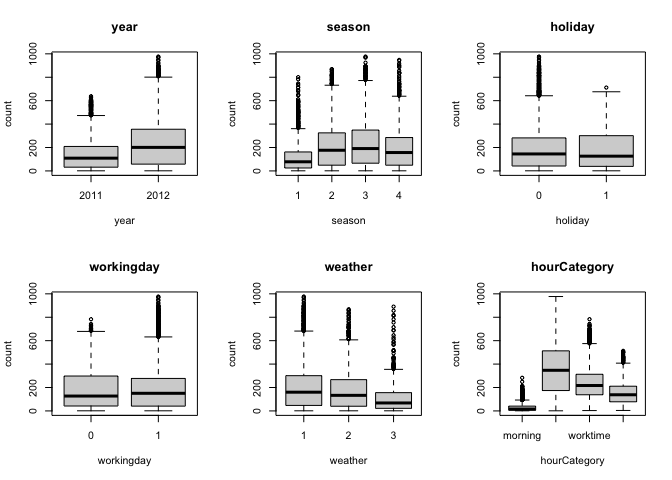
\includegraphics{informe_files/figure-latex/unnamed-chunk-8-1.pdf}

Vemos que a primera vista parece que algunas categorias van a influir
más en la respuesta que otras. Las que tinen boxplots muy similares
entre categorías menos representativas van a ser, como es el caso de
\texttt{holiday} y \texttt{workingday}.

\hypertarget{generaciuxf3n-del-modelo}{%
\section{Generación del modelo}\label{generaciuxf3n-del-modelo}}

\hypertarget{modelo-1---utilizando-todas-las-variables}{%
\subsection{Modelo 1 - Utilizando todas las
variables}\label{modelo-1---utilizando-todas-las-variables}}

\begin{itemize}
\tightlist
\item
  Variables utilizadas: \texttt{year}, \texttt{season},
  \texttt{holiday}, \texttt{workingday}, \texttt{weather},
  \texttt{temp}, \texttt{humidity}, \texttt{windspeed} y
  \texttt{hourCategory}.
\end{itemize}

\begin{longtable}[]{@{}ll@{}}
\toprule
Propiedad & Valores\tabularnewline
\midrule
\endhead
Residual standard error & 111.3\tabularnewline
Multiple R-squared & 0.6276\tabularnewline
p-value & \textless{} 2.2e-16\tabularnewline
\bottomrule
\end{longtable}

\hypertarget{modelo-2---selecciuxf3n-automuxe1tica-de-variables}{%
\subsection{Modelo 2 - Selección automática de
variables}\label{modelo-2---selecciuxf3n-automuxe1tica-de-variables}}

Hemos utilizado el método matemático AIC (Akaike Information Criterion)
para determinar qué conjunto de variables es el óptimo para explicar el
modelo y cualos sería conveniente eliminar. Recordemos que cuanto menor
es el AIC mejor.

\begin{longtable}[]{@{}ll@{}}
\toprule
Variable a eliminar & AIC eliminando la variable\tabularnewline
\midrule
\endhead
\texttt{workingday} & 72472\tabularnewline
\texttt{\textless{}ninguna\textgreater{}} & 72473\tabularnewline
\texttt{windspeed} & 72474\tabularnewline
\texttt{holiday} & 72476\tabularnewline
\texttt{weather} & 72562\tabularnewline
\texttt{humidity} & 72664\tabularnewline
\texttt{season} & 72862\tabularnewline
\texttt{temp} & 73040\tabularnewline
\texttt{year} & 73501\tabularnewline
\texttt{hourCategory} & 77039\tabularnewline
\bottomrule
\end{longtable}

Eliminamos la variable \texttt{workingday} y generamos otro modelo. A
continuación el resultado.

\begin{longtable}[]{@{}ll@{}}
\toprule
Propiedad & Valores\tabularnewline
\midrule
\endhead
Residual standard error & 111.3\tabularnewline
Multiple R-squared & 0.6275\tabularnewline
p-value & \textless{} 2.2e-16\tabularnewline
\bottomrule
\end{longtable}

\begin{itemize}
\tightlist
\item
  Vemos un resultado prácticamente idéntico al del Modelo 1 pero
  utilizando una variable menos.
\end{itemize}

\hypertarget{anuxe1lisis-de-colinealidad-de-las-variables}{%
\subsubsection{Análisis de colinealidad de las
variables}\label{anuxe1lisis-de-colinealidad-de-las-variables}}

Utilizamos el indicador de VIF para analizar la colinealidad de las
variables restantes por si tuviéramos que eliminar alguna más. Buscamos
un valor de VIF \textless{} 5.

\begin{longtable}[]{@{}ll@{}}
\toprule
Variable & VIF\tabularnewline
\midrule
\endhead
year & 1.025830\tabularnewline
season & 3.169114\tabularnewline
holiday & 1.003029\tabularnewline
weather & 1.292185\tabularnewline
temp & 3.083793\tabularnewline
humidity & 1.684752\tabularnewline
windspeed & 1.175091\tabularnewline
hourCategory & 1.319474\tabularnewline
\bottomrule
\end{longtable}

Podemos observar que el indicador VIF de todas las variables se mantiene
por debajo del 5, lo que nos indica que hay poca colinealidad entre las
variables y que no tendríamos que eliminar ninguna.

\hypertarget{validaciuxf3n-de-las-premisas}{%
\subsubsection{Validación de las
premisas}\label{validaciuxf3n-de-las-premisas}}

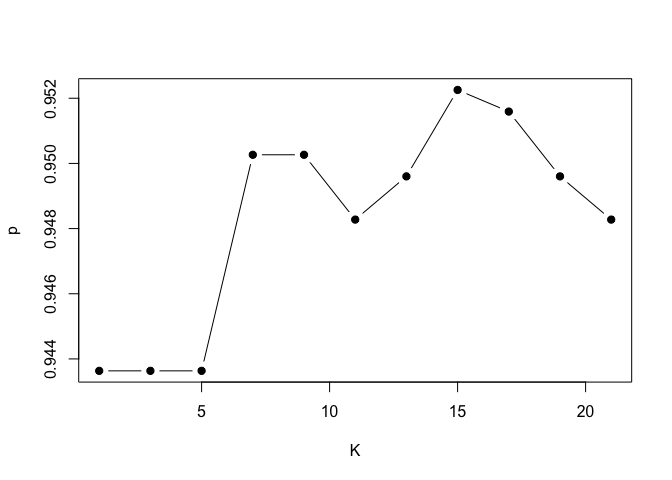
\includegraphics{informe_files/figure-latex/unnamed-chunk-11-1.pdf}
\includegraphics{informe_files/figure-latex/unnamed-chunk-11-2.pdf}

\begin{itemize}
\tightlist
\item
  \textbf{Homocedasticidad}: No se cumple, vemos que la dispersión de
  los residuos no es constante, forman una forma de embudo clara.
\item
  \textbf{Linealidad}: Hay curvatura, tampoco se cumple.
\item
  \textbf{Normalidad de los residuos}: Desviación de la distribución
  normal tanto en valores pequeños como en grandes, no se cumple.
\item
  \textbf{Independencia}: Se cumple, vemos que la dispersión de los
  residuos a lo largo del orden en que aparecen en el conjunto de datos
  es constante.
\end{itemize}

\hypertarget{modelo-3---transformaciuxf3n-de-la-variable-resupesta}{%
\subsection{Modelo 3 - Transformación de la variable
resupesta}\label{modelo-3---transformaciuxf3n-de-la-variable-resupesta}}

Hemos generado dos nuevos modelos utilizando la transformación
logarítmica y la de BoxCox de la variable respuesta. A continuación los
resultados.

\begin{longtable}[]{@{}lll@{}}
\toprule
& Transformación logarítmica & Transformación BoxCox\tabularnewline
\midrule
\endhead
R-squared & 0.7184 & 0.7418\tabularnewline
Residual standard error & 0.7899 & 0.5919\tabularnewline
\bottomrule
\end{longtable}

\begin{itemize}
\tightlist
\item
  En general vemos una mejora sustancial utilizando una transformación
  en la variable respuesta, cualquiera de las dos.
\item
  De las dos transformaciones, nos quedamos con la de BoxCox ya que nos
  da un mejor resultado.
\end{itemize}

\hypertarget{modelo-final---modelo-3}{%
\section{Modelo final - Modelo 3}\label{modelo-final---modelo-3}}

\begin{itemize}
\item
  Variables utilizadas:
  \texttt{year,\ season,\ holiday,\ weather,\ temp,\ humidity,\ windspeed,\ hourCategory}
\item
  Transformaciones:

  \begin{itemize}
  \tightlist
  \item
    BoxCox en la variable respuesta
  \item
    Categorización de la variable hora
  \end{itemize}
\item
  Resultado:

  \begin{longtable}[]{@{}lll@{}}
  \toprule
  Propiedes & Valores &\tabularnewline
  \midrule
  \endhead
  Residual standard error & 0.5919 &\tabularnewline
  Multiple R-squared & 0.7418 &\tabularnewline
  p-value & \textless{} 2.2e-16 &\tabularnewline
  \bottomrule
  \end{longtable}
\item
  Expresión del modelo
\end{itemize}

\begin{verbatim}
## 
## Call:
## lm(formula = countBC ~ year + season + holiday + weather + temp + 
##     humidity + windspeed + hourCategory, data = datos)
## 
## Residuals:
##     Min      1Q  Median      3Q     Max 
## -2.7752 -0.3683  0.0015  0.4019  1.8997 
## 
## Coefficients:
##                        Estimate Std. Error t value Pr(>|t|)    
## (Intercept)           1.5161674  0.0423634  35.790  < 2e-16 ***
## year2012              0.4364839  0.0136742  31.920  < 2e-16 ***
## season2               0.2660031  0.0250530  10.618  < 2e-16 ***
## season3               0.1770850  0.0320088   5.532 3.26e-08 ***
## season4               0.4738698  0.0208005  22.782  < 2e-16 ***
## holiday1             -0.1075865  0.0402854  -2.671  0.00759 ** 
## weather2             -0.0291989  0.0167442  -1.744  0.08123 .  
## weather3             -0.3931704  0.0281752 -13.954  < 2e-16 ***
## temp                  0.0380311  0.0015152  25.100  < 2e-16 ***
## humidity             -0.0056539  0.0004540 -12.455  < 2e-16 ***
## windspeed            -0.0022970  0.0008947  -2.567  0.01027 *  
## hourCategorymoving    2.1240396  0.0203887 104.177  < 2e-16 ***
## hourCategoryworktime  1.6613631  0.0195673  84.905  < 2e-16 ***
## hourCategorynight     1.3035639  0.0211916  61.513  < 2e-16 ***
## ---
## Signif. codes:  0 '***' 0.001 '**' 0.01 '*' 0.05 '.' 0.1 ' ' 1
## 
## Residual standard error: 0.5919 on 7675 degrees of freedom
## Multiple R-squared:  0.7418, Adjusted R-squared:  0.7413 
## F-statistic:  1696 on 13 and 7675 DF,  p-value: < 2.2e-16
\end{verbatim}

\hypertarget{validaciuxf3n-del-modelo}{%
\subsection{Validación del modelo}\label{validaciuxf3n-del-modelo}}

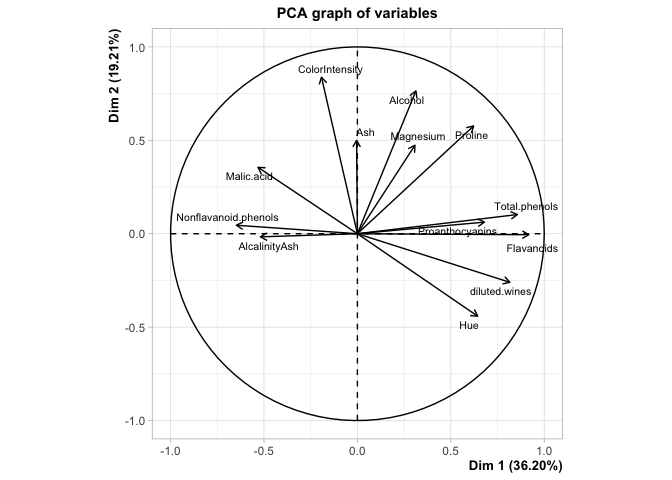
\includegraphics{informe_files/figure-latex/unnamed-chunk-14-1.pdf}
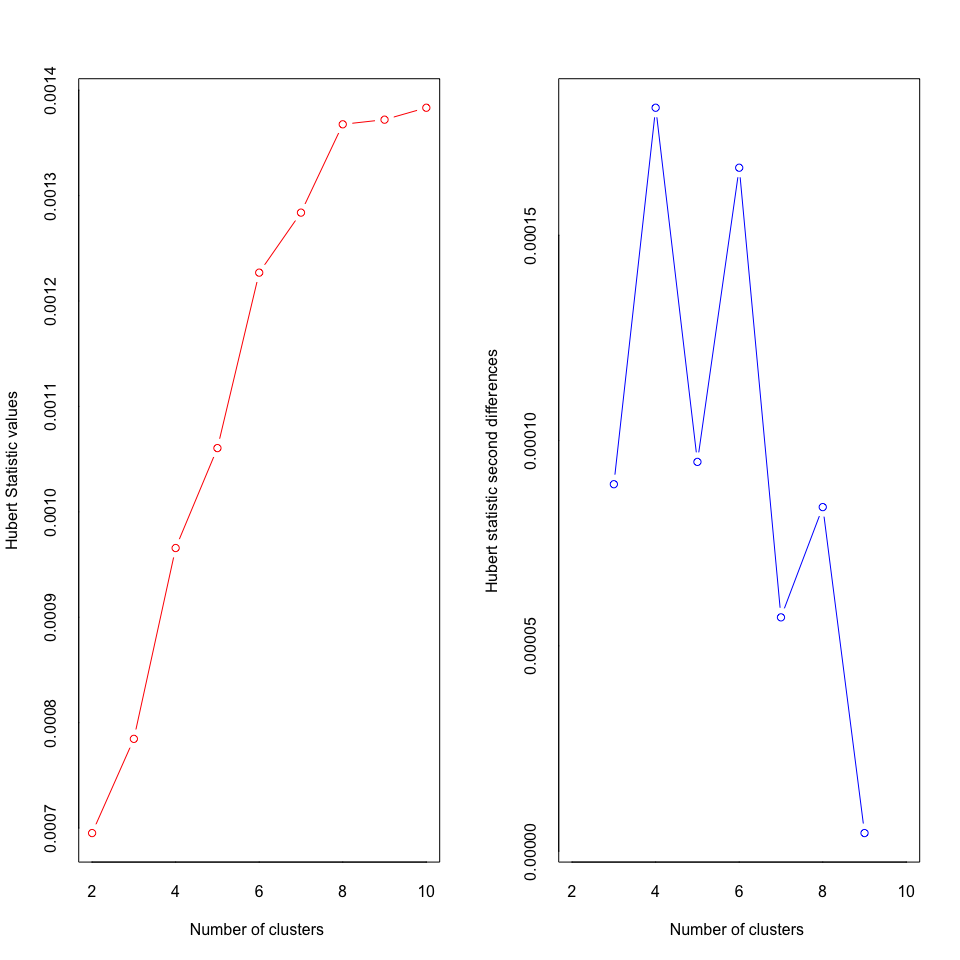
\includegraphics{informe_files/figure-latex/unnamed-chunk-14-2.pdf}

\begin{itemize}
\tightlist
\item
  \textbf{Homocedasticidad}: Se cumple, sigue habiendo más dispersión en
  el centro y en valores más altos que en pequeños, pero ya no tenemos
  la forma de embudo tan destacada que teníamos en el Modelo 2.
\item
  \textbf{Linealidad}: Se cumple, hay curvatura pero muy leve.
\item
  \textbf{Normalidad de los residuos}: Sigue desviándose en valores
  altos pero podríamos considerar que ahora se cumple, ha mejorado
  respecto al Modelo 2.
\item
  \textbf{Independencia}: Se cumple, igual que en el Modelo 2.
\end{itemize}

\hypertarget{efecto-de-las-caracteruxedsticas-sobre-la-variable-respuesta}{%
\subsection{Efecto de las características sobre la variable
respuesta}\label{efecto-de-las-caracteruxedsticas-sobre-la-variable-respuesta}}

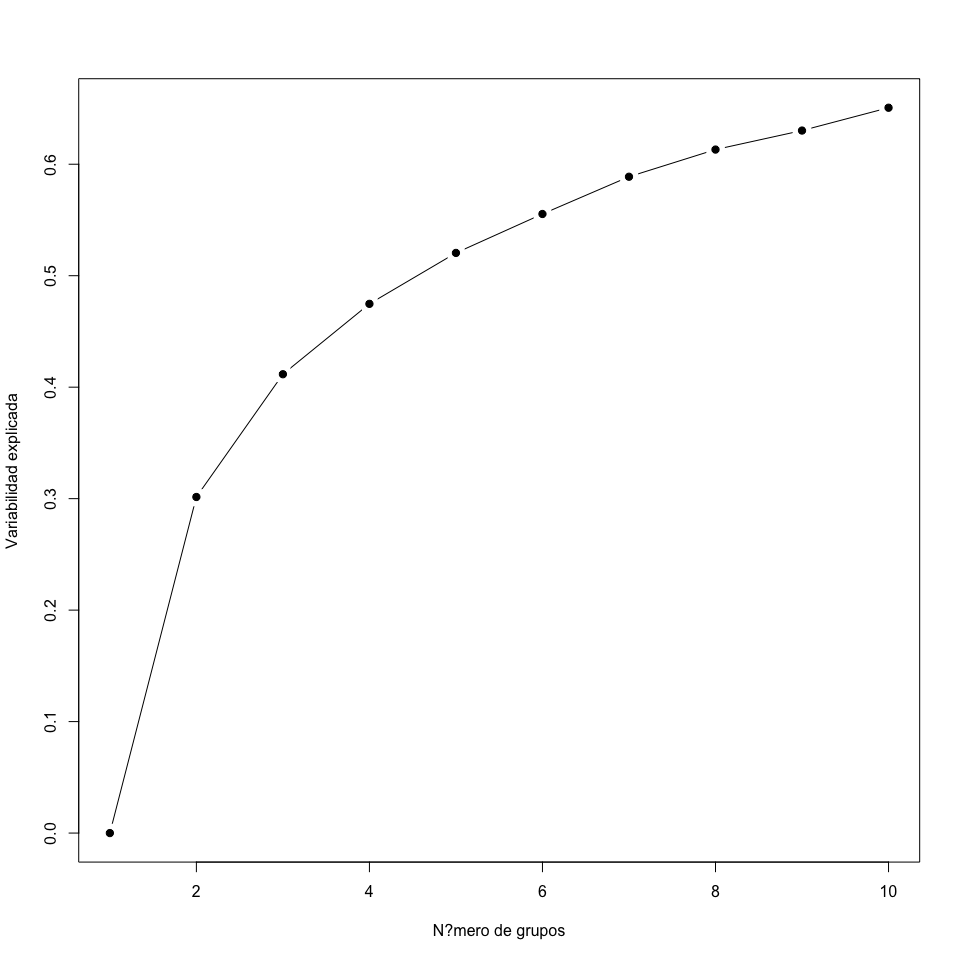
\includegraphics{informe_files/figure-latex/unnamed-chunk-15-1.pdf}

\newpage

\hypertarget{anexos---modelos-descartados}{%
\section{Anexos - Modelos
descartados}\label{anexos---modelos-descartados}}

\hypertarget{modelo-4-transformaciuxf3n-polinuxf3mica}{%
\subsection{Modelo 4: Transformación
polinómica}\label{modelo-4-transformaciuxf3n-polinuxf3mica}}

Hemos realizado una transformación polinómica a las variables numéricas
y generado un nuevo modelo con ellas. Vemos el resultado a continuación.

\begin{itemize}
\item
  Modelo de referencia: Modelo 3
\item
  Transformación añadida: Transformación polinómica de las variables
  \texttt{temp}, \texttt{humidity} y \texttt{windspeed}
\item
  Resultado:

  \begin{longtable}[]{@{}ll@{}}
  \toprule
  Propiedes & Valores\tabularnewline
  \midrule
  \endhead
  Residual standard error & 0.5884\tabularnewline
  Multiple R-squared & 0.7449\tabularnewline
  p-value & \textless{} 2.2e-16\tabularnewline
  \bottomrule
  \end{longtable}
\item
  Vemos que hay una diferencia insignificante respecto al Modelo 3, por
  lo que no vemos que sea necesario utilizar la transformación
  polinómica
\end{itemize}

\hypertarget{modelo-5-eliminar-observaciones-influyentes}{%
\subsection{Modelo 5: Eliminar observaciones
influyentes}\label{modelo-5-eliminar-observaciones-influyentes}}

Analizamos las observaciones influyentes del Modelo 3:

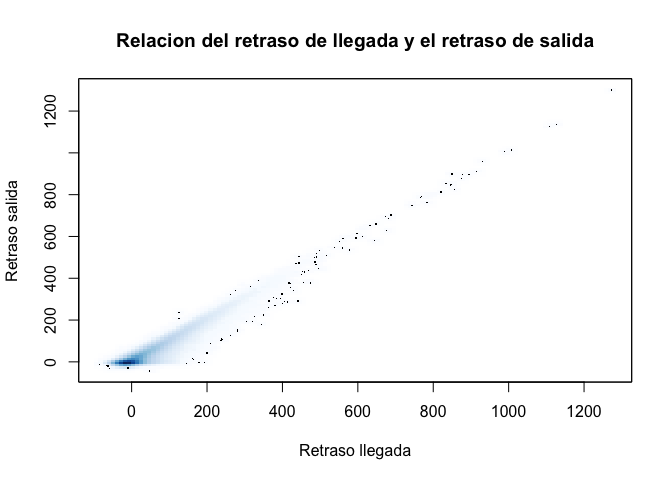
\includegraphics{informe_files/figure-latex/unnamed-chunk-16-1.pdf}

Vemos que las observaciones 2005 y 6737 son las que tienen una distancia
de Cook mayor, por lo que son las más influyentes. A continuación sus
distancias de Cook respectivas:

\begin{longtable}[]{@{}ll@{}}
\toprule
Observación & Distancia de Cook\tabularnewline
\midrule
\endhead
2005 & 0.0050\tabularnewline
6737 & 0.0052\tabularnewline
\bottomrule
\end{longtable}

Eliminamos estas dos observaciones y generamos un nuevo modelo.

\begin{itemize}
\item
  Modelo de referencia: Modelo 3
\item
  Transformación añadida: Eliminación de las observaciones influyentes
  2005 y 6737
\item
  Resultado:

  \begin{longtable}[]{@{}ll@{}}
  \toprule
  Propiedes & Valores\tabularnewline
  \midrule
  \endhead
  Residual standard error & 0.5911\tabularnewline
  Multiple R-squared & 0.7425\tabularnewline
  p-value & \textless{} 2.2e-16\tabularnewline
  \bottomrule
  \end{longtable}
\item
  De nuevo, la diferencia es insignificante respecto el Modelo 3, por lo
  que no interesa hacer esta transformación
\end{itemize}

\end{document}
